\documentclass[11pt]{beamer}
\usetheme{Dresden}
%\usecolortheme{beaver}
\usepackage[utf8]{inputenc}
\usepackage{amsmath}
\usepackage{amsfonts}
\usepackage{amssymb}
\usepackage{graphicx}
\usepackage{verbatim}
\usepackage{listings}
\usepackage{xcolor}
\usepackage{makecell}

\let\OldTexttt\texttt
\renewcommand{\texttt}[1]{\OldTexttt{\color{teal}{#1}}}

\definecolor{mGreen}{rgb}{0,0.6,0}
\definecolor{mGray}{rgb}{0.5,0.5,0.5}
\definecolor{mPurple}{rgb}{0.58,0,0.05}
\definecolor{mGreen2}{rgb}{0.05,0.65,0.05}
\definecolor{mGray2}{rgb}{0.55,0.55,0.55}
\definecolor{mPurple2}{rgb}{0.63,0.05,0.05}
\definecolor{backgroundColour}{rgb}{0.95,0.95,0.92}
\definecolor{backgroundColour2}{rgb}{0.95,0.92,0.95}

\lstdefinestyle{C}{
    backgroundcolor=\color{backgroundColour},   
    commentstyle=\color{mGreen},
    keywordstyle=\color{blue},
    numberstyle=\tiny\color{mGray},
    stringstyle=\color{mPurple},    
    basicstyle=\footnotesize,
    breakatwhitespace=false,         
    breaklines=true,                 
    captionpos=b,                    
    keepspaces=true,                 
    numbers=left,                    
    numbersep=5pt,                  
    showspaces=false,                
    showstringspaces=false,
    showtabs=false,                  
    tabsize=2,
    language=C
}

\lstdefinestyle{Python}{
    backgroundcolor=\color{backgroundColour2},   
    commentstyle=\color{mGreen2},
    keywordstyle=\color{blue},
    numberstyle=\tiny\color{mGray2},
    stringstyle=\color{mPurple2},
    basicstyle=\footnotesize,
    breakatwhitespace=false,         
    breaklines=true,                 
    captionpos=b,                    
    keepspaces=true,                 
    numbers=left,                    
    numbersep=5pt,                  
    showspaces=false,                
    showstringspaces=false,
    showtabs=false,                  
    tabsize=2,
    language=Python
}

\definecolor{eggplant}{rgb}{0.5, 0.25, 0.5} % UBC Blue (primary)

\usecolortheme[named=eggplant]{structure}

\author{NCC Moore}
\title{Topic 13 - The C Preprocessor and Miscellaneous Errata}
%\setbeamercovered{transparent} 
%\setbeamertemplate{navigation symbols}{} 
%\logo{} 
\institute{McMaster University} 
\date{Summer 2021} 
\subject{COMPSCI 1XC3 - Computer Science Practice and Experience:
Development Basics} 
\stepcounter{section}
\begin{document}

\begin{frame}
\center
COMPSCI 1XC3 - Computer Science Practice and Experience:
Development Basics
\titlepage
Adapted from Chapters 13 and 14 of C: How to Program 8th ed., Deitel \& Deitel
\end{frame}

\begin{frame}
\tableofcontents
\end{frame}

\section[Preproc]{Preprocessor Directives}
\begin{frame}{So what's left?}
Not much! We need to go over some of the advanced preprocessor commands:
\begin{itemize}
\item \texttt{\#define}
\item \texttt{\#undef}
\item \texttt{\#if} and \texttt{\#endif}
\item \texttt{\#error} and \texttt{\#pragma}
\item \texttt{\#line}
\end{itemize}
The C preprocessor is responsible for handling all of the operations that need to occur before a source file can be tokenized, an abstract syntax tree produced, and an executable generated.
\begin{itemize}
\item Comments must be removed
\item Preprocessor directives must be processed.
\begin{itemize}
\item A preprocessor directive is some manipulation of the text of the source file.  
\end{itemize}
\end{itemize}
\end{frame}

\begin{frame}[fragile=singleslide]{Macro, Macro Man! (Reprisal)}
At the beginning of the course we explained how macros can set symbolic constants, but we can do more with them than just specifying the size of an array! 
\begin{lstlisting}[style=C]
#define <identifier> <replacement text>
\end{lstlisting}
\begin{itemize}
\item Remember that a macro is a \emph{character substitution operation}
\item This means that a macro can be used to insert \emph{anything} into a C source file. Including:
\begin{itemize}
\item Semicolons and curly braces, complete or partial expressions, assignments, argument lists and function calls
\end{itemize}
\item Macros have no grammatical limitations, though the substitutions they make must result in grammatically correct C code. 
\item It is recommended to keep these substitutions to one line.
\item Macros are named in all-caps by convention.
\end{itemize}
\end{frame}

\begin{frame}[fragile=singleslide]{Macro, Macro Man! (Reprisal, cont.)}
\begin{lstlisting}[style=C]
// A syntactically correct C program: 
#include<stdio.h>

#define BEGIN (){
#define TWICE(x) x x
#define INT_PRINT(x) printf("%d\n", x);
#define AREA(x,y) ((x)*(y))

int main BEGIN
	if (1 == 1) {
		INT_PRINT(AREA(8,10));
TWICE(})
\end{lstlisting}
\hrule
\begin{verbatim}
80
\end{verbatim}
\end{frame}

\begin{frame}[fragile=singleslide]{Macros with Arguments!}
You may have noticed the program on the previous slide contained macros with a function-like construction.
\begin{itemize}
\item Yes! You can make your macros take arguments! 
\item The process somewhat resembles lambdas in Python:
\end{itemize}
\begin{lstlisting}[style=Python]
(lambda x y : x*y)(8,10)
\end{lstlisting}
\begin{itemize}
\item The main difference of course is that we are performing \emph{character substitutions only}, so the arguments to a pragma may be \emph{any group of characters}, so long as the operation results in valid C code.  
\item For example, the macro \texttt{TWICE(x) x x} takes the input \texttt{x} and inserts two of them into the file.  
\item This is used to duplicate the closing curly brace, ending both \texttt{main} and it's if-statement.  
\end{itemize}
\end{frame}

\begin{frame}[fragile=singleslide]{Undefined Reference}
If you want to restrict the applicability of your macro, you can use the following to remove macros:
\begin{lstlisting}[style=C]
#undef <identifier>
\end{lstlisting}
\begin{itemize}
\item Remember that macros are also imported when you include a library or one of your own source files.  
\item By using \texttt{\#undef}, you can prevent macros you define in one file from being applied to another.  
\item Once a macro has been undefined, it can subsequently be redefined, so it can also be useful if you want a macro to perform different substitutions in different parts of your source file.
\begin{itemize}
\item The above does not seem an advisable use-case, as it seems rather spaghetti-code-like.
\end{itemize}
\end{itemize}
\end{frame}

\begin{frame}[fragile=singleslide]{Shampoo and Conditioner}
We can hide code from the compiler conditionally using \texttt{\#if} and \texttt{\#endif}
\begin{lstlisting}[style=C]
#if <condition>
Code which may be deleted
#endif
\end{lstlisting}
\begin{itemize}
\item Any code between \texttt{\#if} and \texttt{\#endif} will be deleted if the condition evaluates to 0, and will be kept otherwise.
\item The conditional expression must have integral type and can include only integer constants, character constants, and the ``defined'' operator.
\begin{itemize}
\item Remember! This command is being executed before your program compiles. As such, functions, variables, enumerations, and typedefs should not be used! 
\item Best to stick to Macros, integer literals and the standard operators.  
\end{itemize}
\end{itemize}
\end{frame}

\begin{frame}{When to be Iffy}
Common use-cases of \texttt{\#if} includes:
\begin{itemize}
\item Preventing a header file from being included multiple times in the same project.
\item Giving a program a debug mode.
\begin{itemize}
\item Typically, in debug mode a program will execute many printf() statements which reveal internal data, or generate a log file.
\end{itemize}
\item Setting different constants / executing different statements, depending on system-defined values.
\begin{itemize}
\item This could be the word size of the processor, the version number of the operating system, or any number of things.  
\item This assumes the program will be compiled from source on multiple different systems.  
\end{itemize}
\end{itemize}
\end{frame}

\begin{frame}{If Variants}
Here are some quality of life improvements! 
\begin{itemize}
\item The \texttt{defined(<Macro>)} operator returns 1 if the specified macro is defined, 0 otherwise.
\item \texttt{\#elif} and \texttt{\#else} may be used in the same way as \texttt{else if} and \texttt{if} to create additional branches.
\item \texttt{\#ifdef x} is shorthand for \texttt{\#if defined(x)}
\item \texttt{\#ifndef x} is shorthand for \texttt{\#if !defined(x)}
\end{itemize}
You can also use \texttt{\#if} to comment out blocks of code.
\begin{itemize}
\item Using \texttt{/*} and \texttt{*/} doesn't allow for nesting, but \texttt{\#if} and \texttt{\#endif} do!
\end{itemize}
\end{frame}

\begin{frame}{Miscellaneous Directives}
\begin{itemize}
\item \texttt{\#error <tokens>} prints an error message
\begin{itemize}
\item What the error message says depends on your system and C implementation
\item Halts compilation upon execution.
\end{itemize}
\item \texttt{\#pragma <tokens>} performs miscellaneous commands
\begin{itemize}
\item Which pragmas are available depends on your system and C implementation.
\item Using pragmas may make your code less portable! 
\end{itemize}
\item \texttt{\#line <integer>} manually changes the line number of the source file.
\begin{itemize}
\item Generally used to generate more meaningful compiler warnings and errors.
\end{itemize}
\end{itemize}
\end{frame}

\section[signals]{Signal Handling}
\begin{frame}{Sending out Signals}
\center
\large{C DOES NOT SUPPORT EXCEPTION HANDLING}
\flushleft
\begin{itemize}
\item It handles \textbf{signals} instead, which, as with most things in C, are not quite the same thing.
\item For each process, the operating system maintains 2 integers which indicate the status of various signals.
\begin{itemize}
\item One is for pending signals
\item The other blocks pending signals.
\end{itemize}
\item The signal handling library of C is \texttt{<signal.h>}
\item This library contains a number of defined values, which indicate various signal types.  
\item Most of these signals correspond closely to the types of exceptions you saw in python.
\end{itemize}
\end{frame}

\begin{frame}{Signal Types}
\center
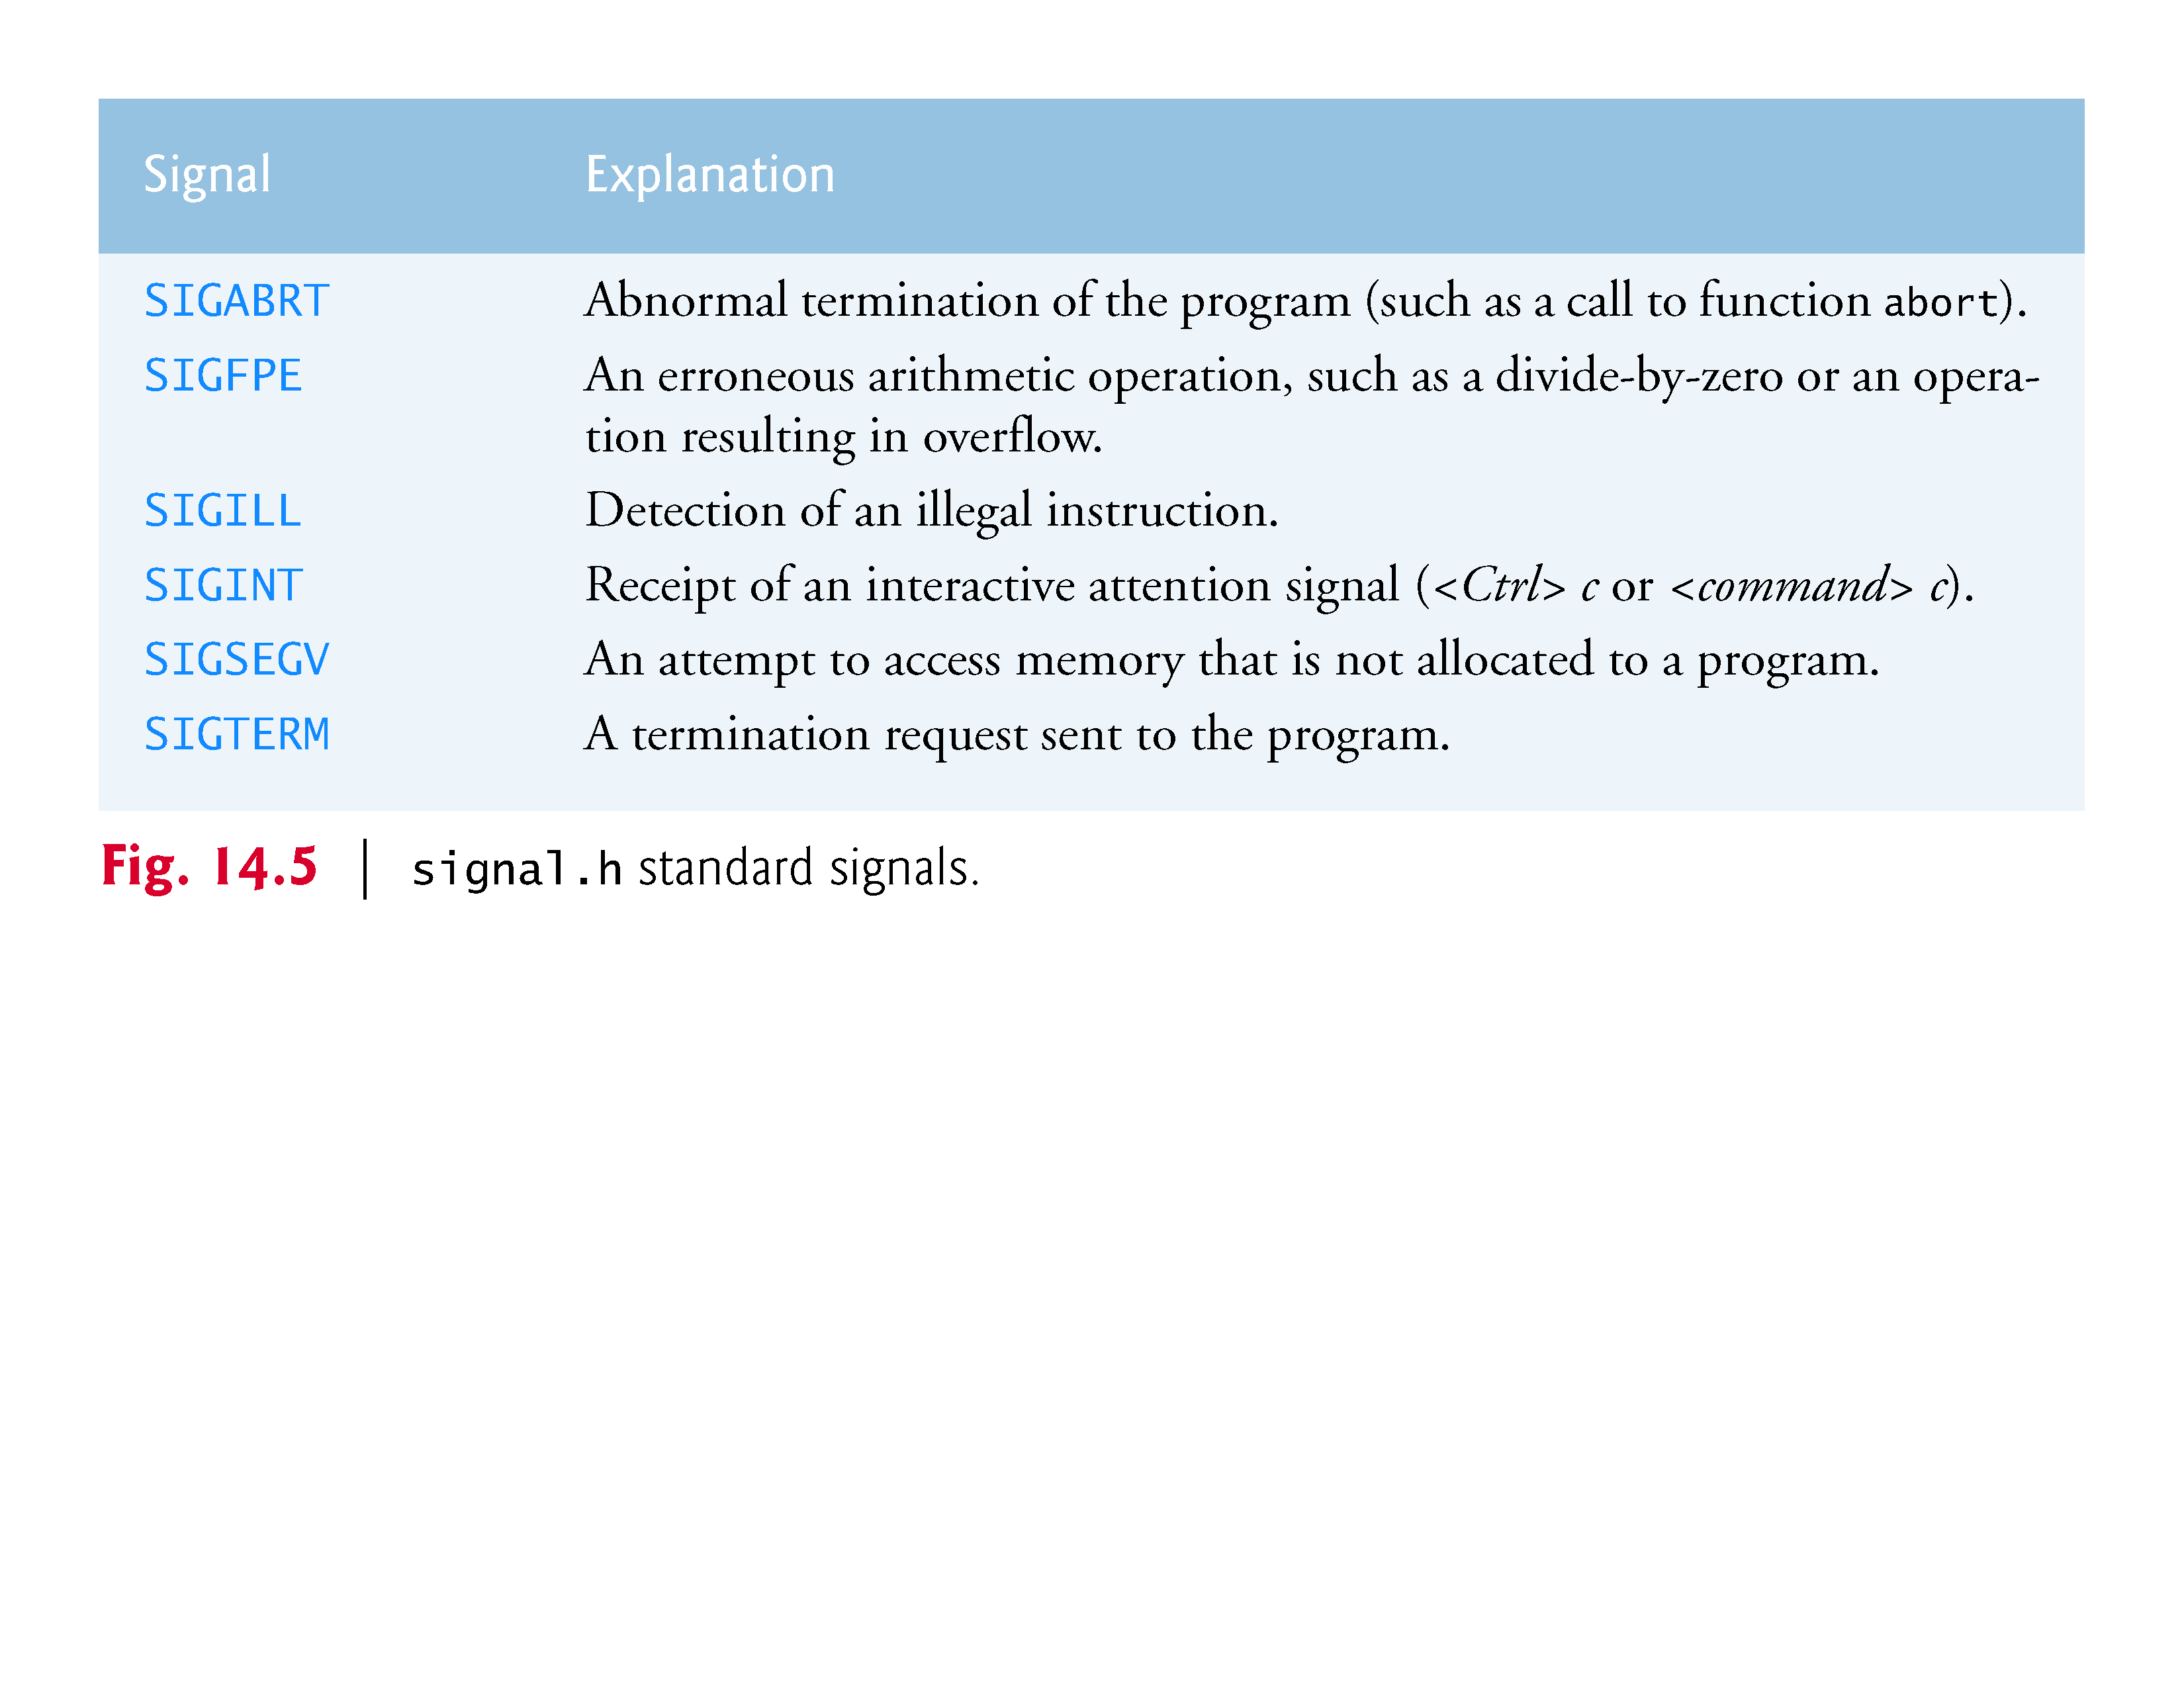
\includegraphics[scale=0.35]{signals.png}
\end{frame}

\begin{frame}[fragile=singleslide]{Not Handling Not Exceptions}
\begin{itemize}
\item In order to handle a signal, you must register a function to activate for an incoming signal of a particular type.
\end{itemize}
\begin{lstlisting}[style=C]
signal(<signal>, <function pointer>)
\end{lstlisting}
\begin{itemize}
\item The \texttt{signal()} function is provided in \texttt{<signal.h>}.
\item The function associates an incoming signal type with a function. 
\item  If the signal is received during program execution, execution is paused, and the function is immediately entered.  
\item Once the function is terminated, the association between signal and function is broken.
\begin{itemize}
\item Fortunately, it is possible to call \texttt{signal()} from within the signal-handling function.  
\end{itemize}
\end{itemize}
\end{frame}

\begin{frame}[fragile=singleslide]{A Somewhat Long but Humorous Example}
\begin{lstlisting}[style=C]
#include<stdio.h>
#include<signal.h>
#include <unistd.h>

int finish = 0;

void handle_sigint (int signal_Value) {
	finish = 1;
}

int main() {
	signal(SIGINT, handle_sigint); 
	printf("Let me tell you a joke...\n");
    sleep(1); 
//...
\end{lstlisting}    
\end{frame}

\begin{frame}[fragile=singleslide]{A Somewhat Long but Humorous Example (cont.)}
\begin{lstlisting}[style=C]
//...
    while (1) 
    { 
    	if (finish) {
    		printf("  A: Knock Knock\n"); sleep(1); 
    	    printf("  B: Who's there?\n"); sleep(1);
    	    printf("  A: Orange.\n"); sleep(1);
    	    printf("  B: Orange who?\n"); sleep(1);
	        printf("  A: Orange you glad I didn't say Banana?\n"); sleep(1);
	        break;
    	} else {
    	    printf("  A: Knock Knock\n"); sleep(1); 
    	    printf("  B: Who's there?\n"); sleep(1);
    	    printf("  A: Banana.\n"); sleep(1);
    	    printf("  B: Banana who?\n"); sleep(1);
//...
\end{lstlisting}    
\end{frame}

\begin{frame}[fragile=singleslide]{A Somewhat Long but Humorous Example (cont.)}
\begin{lstlisting}[style=C]
/...
	    printf("  A: Ba-na\n"); sleep(1);
        	printf("        na\n"); sleep(1);
        	printf("        na\n"); sleep(1);
        	printf("        na\n"); sleep(1);
        	printf("        na-na\n"); sleep(1);
        }
    } 
    return 0; 
}
\end{lstlisting}
\center
Cue Demo! 
\end{frame}

\begin{frame}
\center
Thus concludes our discussion of the C programming language.
\begin{columns}
\begin{column}{0.25\textwidth}
\center
\scalebox{-1}[1]{
\includegraphics[scale=0.25]{party.png}}
\end{column}
\begin{column}{0.5\textwidth}
\center
\LARGE{CONGRATULATIONS YOU MAGNIFICENT HUMAN BEINGS} \\
\end{column}
\begin{column}{0.25\textwidth}
\center

\includegraphics[scale=0.25]{party.png}
\end{column}
\end{columns}
\vspace{1em}

\includegraphics[scale=0.2]{weredone.jpg}
\end{frame}

\end{document}